\subsection{Рекуррентные и интегральные соотношения для решений уравнения Бесселя. Ортогональность функций Бесселя. Ряды Фурье – Бесселя.}
\label{sec:bessel}
%ref: Свешников, стр. 66 - 75
%aut: Денис

%TODO Сократить
Функции Бесселя возникают при решении уравнений, связанных с оператором Лапласа $\Delta$ на плоскости,
\[
-\Delta u(x, y) \equiv-\frac{\partial^{2} u}{\partial x^{2}}-\frac{\partial^{2} u}{\partial y^{2}}=\lambda u+f(x, y) .
\]

Действительно, в полярных координатах $(r, \varphi)$, это уравнение принимает вид
\[
-\frac{1}{r} \frac{\partial}{\partial r}\left(r \frac{\partial \widetilde{u}}{\partial r}\right)-\frac{1}{r^{2}} \frac{\partial^{2} \widetilde{u}}{\partial \varphi^{2}}=\lambda \widetilde{u}+\widetilde{f}(r, \varphi), \quad \widetilde{u}(r, \varphi)=u(r \cos \varphi, r \sin \varphi) .
\]

Если решение $\widetilde{u}(r)$ не зависит от $\varphi$, то последнее уравнение при $f=0$ принимает вид
\[
u^{\prime \prime}(r)+\frac{1}{r} u^{\prime}(r)+\lambda u(r)=0
\]

и является частным случаем \textbf{уравнения Бесселя}
\[
x^{2} u^{\prime \prime}+x u^{\prime}+\left(x^{2}-v^{2}\right) u=0 .
\]

\textbf{Реккурентное представление}

Рассмотрим функцию
\[
J_v(x) = \sum_{k=0}^{\infty}\frac{(-1)^k}{\Gamma(k+v+1)\Gamma(k+1)} \left(\frac{x}{2}\right)^{2k+v}
\]

называемую \textbf{функцией Бесселя}. Путем прямой проверки легко убедиться в справедливости соотношений
\[
\frac{d}{d x}\left(\frac{J_{v}(x)}{x^{v}}\right)=-\frac{J_{v+1}(x)}{x^{v}}
\]

и
\[
\frac{d}{d x}\left(x^{v} J_{v}(x)\right)=x^{v} J_{v-1}(x) .
\]

Докажем, например, первую формулу:
\[
\begin{aligned}
	x^{v} \frac{d}{d x}\left(\frac{J_{v}(x)}{x^{v}}\right)=x^{v} \frac{d}{d x} \sum_{k==0}^{\infty} \frac{(-1)^{k}}{\Gamma(k+1) \Gamma(k+v+1)} \frac{x^{2 k}}{2^{2 k+v}}= \\
	=\left(\frac{x}{2}\right)^{v} \sum_{k=0}^{\infty} \frac{(-1)^{k} 2 k x^{2 k-1}}{k ! \Gamma(k+v+1) 2^{2 k}}=\sum_{k=1}^{\infty} \frac{(-1)^{k}}{\Gamma(k) \Gamma(k+v+1)}\left(\frac{x}{2}\right)^{2 k+(v-1)} .
\end{aligned}
\]

Введем новый индекс суммирования $l=k-1$ :
\[
\begin{aligned}
	x^{v} \frac{d}{d x}\left(\frac{J_{v}(x)}{x^{v}}\right)=-\sum_{l=0}^{\infty} \frac{(-1)^{l}}{\Gamma(l+1) \Gamma}\left(l+\frac{(v+1)+1)}{\left(\frac{x}{2}\right.}\right)^{2 l+(v+1)}= -J_{v+1}(x),
\end{aligned}
\]

Аналогично доказывается вторая формула.

Произведем дифференцирование обеих формул:
\[
\begin{aligned}
	\frac{v^{\prime}}{x} J_{v}(x)-J_{v}^{\prime}(x)=J_{v+1}(x), \\
	\frac{v}{x} J_{v}(x)+J_{v}^{\prime}(x)=J_{v-1}(x) .
\end{aligned}
\]

Складывая две последние формулы, получим полезную рекуррентную формулу
\[
J_{v+1}(x)=\frac{2 v}{x} J_{v}(x)-J_{v-1}(x),
\]

а вычитая, получим формулу для производной
\[
J_{v}^{\prime}(x)=\frac{1}{2}\left\{J_{v-1}(x)-J_{v+1}(x)\right\} .
\]

\textbf{Интегральное представление}

Воспоьзовавшись теоремой умножения Гамма-функция и представлением в виде интеграла Римана-Ханкеля, имеем:

\[
\frac{1}{\Gamma(z+1)} = \frac{e^{i\pi z}}{2 \pi i}\int_{\gamma} e^{-t} t^{-z-1}dl
\]

где $\gamma$ - любой контур на комплексной плоскости t, обходящий точку t=0 против часовой стрелки и концы которого уходят на бесконечность вдоль положительной вещественной оси.

положим $z = k + v$, подставим в формулу для функции Бесселя, меняя порядок сумирования и интегрирования, получим:

\[
\begin{aligned}
	J_{v}(x)=\sum_{k=0}^{\infty} \frac{(-1)^{k}}{\Gamma(k+1) \Gamma(k+v+1)}\left(\frac{x}{2}\right)^{2 k+v}= \\
	=\frac{e^{i \pi v}}{2 \pi i} \int_{\gamma} e^{-t}\left(\frac{x}{2 t}\right)^{v} \sum_{k=0}^{\infty} \frac{\left(\frac{x_{1}^{2}}{4 t}\right)^{k}}{k !} \frac{d t}{t}= \\
	=\frac{e^{i \pi v}}{2 \pi i} \int_{\gamma}\left(\frac{x}{2 t}\right)^{v} e^{\frac{x^{2}}{4 t}-t} \frac{d t}{t} .
\end{aligned}
\]

Пользуясь теоремой Коши, выберем в качестве $\gamma$ контур, состоящий из луча $\left(+\infty, \frac{x}{2}\right)$ на верхнем берегу разреза вдоль положительной части вещественной оси, окружности с центром $t=0$ и радиусом $\frac{x}{2}$, которая обходится против часовой стрелки, и луча $\left(\frac{x}{2},+\infty\right)$ на нижнем берегу разреза .

Сделаем замену $t=\frac{x}{2} e^{-i(\zeta-\pi)}$. При этом контур $\gamma$ на комплексной плоскости $t=t_{1}+i t_{2}$ перейдет в контур $C_{0}$ - на плоскости $\zeta=\zeta_{1}+i \zeta_{2}$ с соответствующим направлением обхода. Учитывая, что
\[
\begin{aligned}
	d t=-i t d \zeta, \frac{x}{2 t}=e^{i(\zeta-\pi)}, \\
	\frac{x^{2}}{4 t}-t=\left(e^{i 2(\zeta-\pi)}-1\right) t= \\
	=\frac{x}{2}\left\{e^{i(\zeta-\pi)}-e^{-i(\zeta-\pi)}\right\}=i x \sin (\zeta-\pi)=-i x \sin \zeta,
\end{aligned}
\]

и используя формулу страницей выше, получим
\[
J_{v}(x)=-\frac{1}{2 \pi} \int_{C_{0}^{-}} e^{-i x \sin \zeta+i v\zeta} d \zeta.
\]

Поменяв в последней формуле направление обхода контура $C_{0}^{-}$ и обозначив полученный контур через $C_{0}^{+}$, получим
\[
J_{v}(x)=\frac{1}{2 \pi} \int_{C_{0}^{+}} e^{-i x \sin \zeta +i v\zeta} d \zeta .
\]

Эта формула носит название интегрального представления Зоммерфельда для функции Бесселя. Сделав в ней замену
\[
\begin{array}{l}
	\xi=\zeta_{2} \text { при } \zeta= \pm \pi+i\zeta_2, \\
	\alpha=\zeta_{1} \text { при } \zeta=\zeta_{1},
\end{array}
\]

получим формулу
\[
J_{v}(x)=\frac{1}{2 \pi} \int_{-\pi}^{\pi} e^{-i x \sin \alpha+i v \alpha} d \alpha-\frac{\sin v \pi}{\pi} \int_{0}^{\infty} e^{-x \operatorname{sh} \xi-v \xi} d \xi .
\]

В частности, при $v=n$
\[
J_{n}(x)=\frac{1}{2 \pi} \int_{-\pi}^{\tau} e^{-i x \sin \alpha+i n \alpha} d \alpha .
\]


Сделаем в последней формуле замену $\alpha=\varphi+\frac{\pi}{2}$. Тогда, поскольку подынтегральная функция является периодической и интегрирование можно производить по любому промежутку длнной $2 \pi$, получим вторую интегральную формулу для функции $J_{n}(x)$ :
\[
J_{n}(x)=\frac{i^{n}}{2 \pi} \int_{-\pi}^{\pi} e^{-i x \cos \varphi+i n \varphi} d \varphi .
\]

Отсюда следует, что для плоской волны $e^{-i x \cos q}$ имеет место разложение в ряд Фурье
\[
e^{-i x \cos \varphi}=\sum_{n=-\infty}^{\infty}(-i)^{n} J_{n}(x) e^{-i n \varphi},
\]

поскольку формула выше является формулой для коэффициентов Фурье этого разложения.

\paragraph{Функции Бесселя второго рода.}
%TODO
Обозначаются $ Y_n(x) $ или $ N_n(x) $.

\paragraph{Некоторые свойства функций Бесселя.}
Изобразим функции Бесселя первого и второго рода соответственно.
% \begin{figure}[H]
%   \centering
%   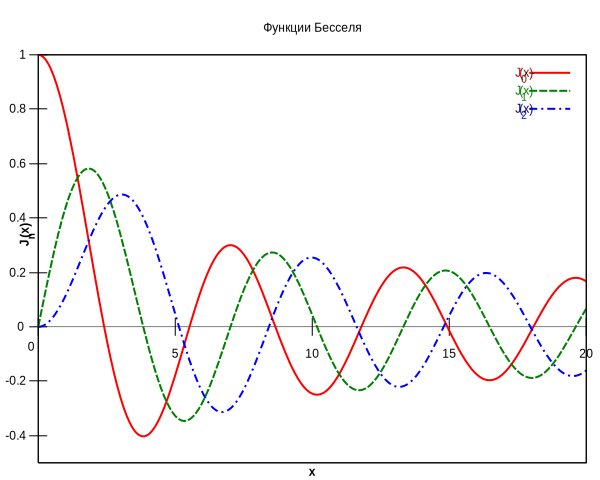
\includegraphics[width=0.8\textwidth]{img/bessel1-plot.svg}
% \end{figure}

\includesvg{bessel1-plot}

\includesvg{bessel2-plot}

По этим графикам видно\footnote{Лучше, конечно, доказать это аналитически.}, что
функция Бесселя второго рода не ограничена в нуле. Обе функции имеют счётное
количество корней --- то же касается и их производных. Функция $ J_n(x) $ при $
x\to\infty$ стремится к нулю. График функции Бесселя похож на
синусоиду, колебания которой затухают пропорционально $1/\sqrt{x}$, хотя на самом деле нули функции расположены не периодично (однако расстояние между двумя последовательными нулями стремится к 
$\pi$ при $x\to \infty $).
